\section{Supernova forward-model analysis}

The methodology used to generate supernova in the self consistent simulations and DC PV are different as we have mentioned earlier. We want to ensure that we can 
quantify any systematic biases introduced by those differences. To do this we start by generating an intial density field using BORG $\delta^{\text{BORG}}_{IC}$ using a 
Planck18 cosmology (\cite{Planck_2018_params}) and known bulk flow $\mathbf{V}$. The configuration of the generated field is given in Table \ref{tab:borg_nbody}. 
We then let that field evolve using the LPT gravity model giving us the evolved density field 
$\delta^{\text{BORG}}_{F}$ and velocity field $\mathbf{v}^{\text{BORG}}_{IC}$. The ZTF simulations are designed to generate the supernovae on top of an N-body simulation, so 
from the evolved density field we create a "synthetic" N-body simulation. The simplest way to do so would be taking each voxel-$i$ and generate within it $N_i$ particles proportional 
to $(1+\lceil \delta^{\text{BORG}}_{F}\rceil )_i$ where $i$ denotes the voxel's index. We take the cieling of the evolved density field to ensure we get an integer number of 
particles and to have at least 1 particle in empty voxels. We also generate less particles than the Uchuu simulation, around 200 million, due to memory and storage limiations. \\

\begin{table}[ht]
    \centering
    \caption{Set of parameters used to generate the "synthetic" N-body BORG simulation.}
    \label{tab:borg_nbody}
    \begin{tabular}{|l|c|}
        \hline
        Parameters & Values \\
        \hline
        Gravity model & LPT \\
        $V_x$ & 0 km/s \\
        $V_y$ & 0 km/s \\
        $V_z$ & 0 km/s \\
        $\Omega_m$ & 0.315 \\
        $\sigma_8$ & 0.81 \\
        \hline
    \end{tabular}
\end{table}
We then use this "synthetic" N-body simulation to generate ZTF-like supernova and then evaluate the BORG-supernova likelihood described in Equation (ref) 
while varying the cosmological and model parameters in BORG. Essentially creating a likelihood profile for each parameter. This is particularly important not just to 
determine whether the ZTF-like supernova simulations introduce systematic biases in BORG but also help us understand how we can relate some of the BORG-supernova model packagesarameters, 
such as $\alpha$ to the ZTF simulations as they are not explicitly specified. \\

We obtain the following likelihood profiles for 1 synthetic N-body simulation in Figures \ref{fig:cosmo_lpt_L}, \ref{fig:params1_lpt_L}, \ref{fig:params2_lpt_L} and \ref{fig:params3_lpt_L}. We notice that the cosmological parameters $\Omega_m$ and $\sigma_8$ are unbiased and we recover the 
input cosmology. The bulk flow $V$ parameters are compatible with 0 km/s, indicating that no additional bulk flow is added with the ZTF simulation. The bias model parameter $\alpha$ 
seems to prefer values around $0.9 -1.0$. This is not unexpected, if we assume that the ZTF supernova are generated where there are dark matter particles without a preference on whether 
then the number of supernovae would simply scale as $\delta_F$. The velocity dispersion is prefered around $150$ km/s with a large scatter. Measurements from (ref smth regarding sigv like velocity olympics) 
getting such values is possible and is indeed physical. The $\mu_A$ parameter seem to prefer a value of $1.024$ indicating that an offset of about $2.4\%$ regarding how distances are described in BORG. 
(check where does it come from but it is not an issue for our needs).

\begin{figure}
    \centering
    \begin{subfigure}{0.45\textwidth}
        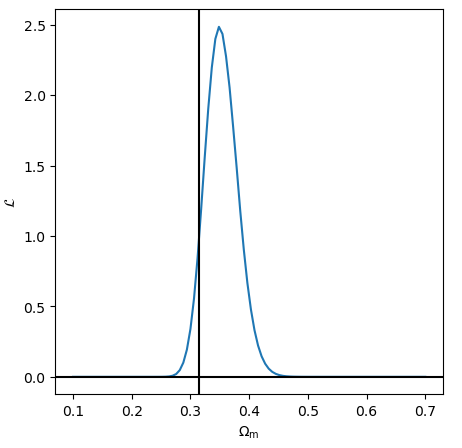
\includegraphics[width=\textwidth]{MainLayout/BORG_chapter/figures/omega_m_L.png}
        \caption{Likelihood profile for $\Omega_m$}
        \label{fig:omega_m_lpt_L}
    \end{subfigure}
    \hfill
    \begin{subfigure}{0.45\textwidth}
        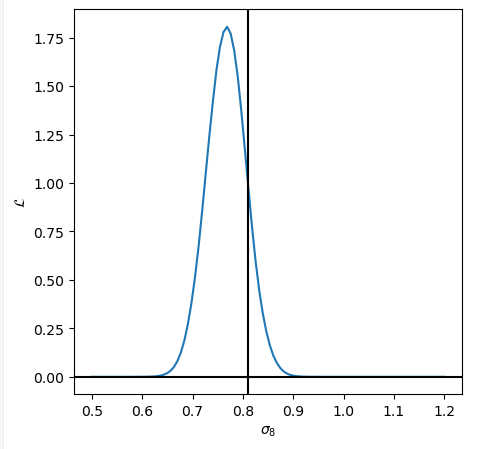
\includegraphics[width=\textwidth]{MainLayout/BORG_chapter/figures/sigma_8_L.png}
        \caption{Likelihood profile for $\sigma_8$}
        \label{fig:sigma8_lpt_L}
    \end{subfigure}
    \caption{Likelihood profiles of the cosmological parameters for a synthetic N-body simulation generated with LPT}
    \label{fig:cosmo_lpt_L}
\end{figure}

\begin{figure}
    \centering
    \begin{subfigure}{0.45\textwidth}
        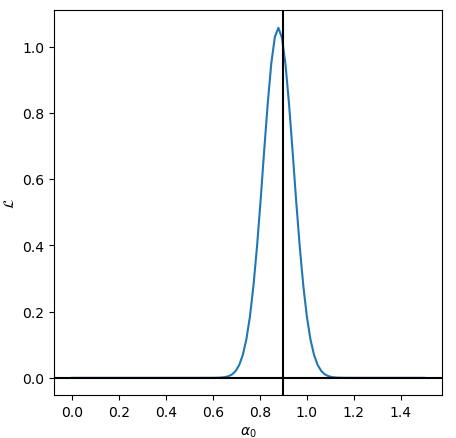
\includegraphics[width=\textwidth]{MainLayout/BORG_chapter/figures/alpha_L.png}
        \caption{Likelihood profile for $\alpha$}
        \label{fig:alpha_lpt_L}
    \end{subfigure}
    \hfill
    \begin{subfigure}{0.45\textwidth}
        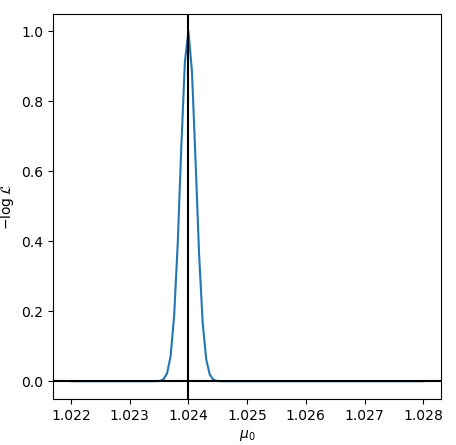
\includegraphics[width=\textwidth]{MainLayout/BORG_chapter/figures/muA_L.png}
        \caption{Likelihood profile for $\mu_A$}
        \label{fig:muA_lpt_L}
    \end{subfigure}
    \caption{Likelihood profiles of $\alpha$ and $\mu_A$ for a synthetic N-body simulation generated with LPT}
    \label{fig:params1_lpt_L}
\end{figure}

\begin{figure}
    \centering
    \begin{subfigure}{0.45\textwidth}
        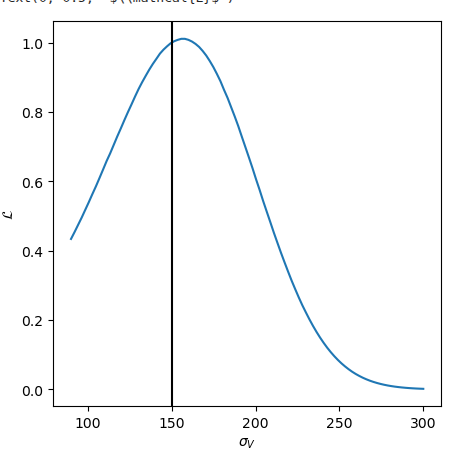
\includegraphics[width=\textwidth]{MainLayout/BORG_chapter/figures/sigma_v_L.png}
        \caption{Likelihood profile for $\sigma_v$}
        \label{fig:sigma_v_lpt_L}
    \end{subfigure}
    \hfill
    \begin{subfigure}{0.45\textwidth}
        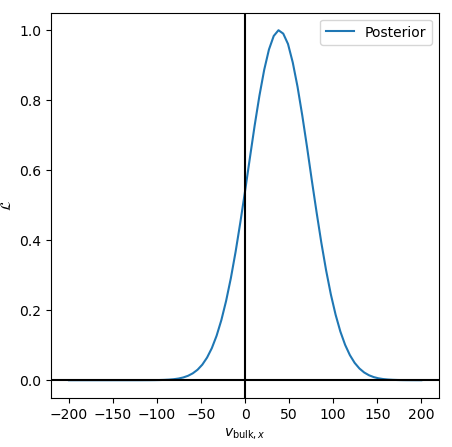
\includegraphics[width=\textwidth]{MainLayout/BORG_chapter/figures/bulk_x_L.png}
        \caption{Likelihood profile for $V_x$}
        \label{fig:Vx_lpt_L}
    \end{subfigure}
    \caption{Likelihood profiles $\sigma_v$ and $V_x$ for a synthetic N-body simulation generated with LPT}
    \label{fig:params2_lpt_L}
\end{figure}

\begin{figure}
    \centering
    \begin{subfigure}{0.45\textwidth}
        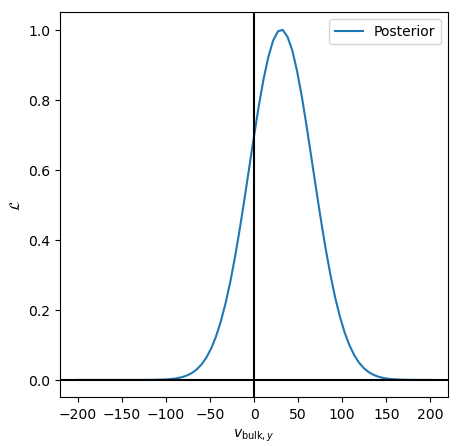
\includegraphics[width=\textwidth]{MainLayout/BORG_chapter/figures/bulk_y_L.png}
        \caption{Likelihood profile for $V_y$}
        \label{fig:Vy_lpt_L}
    \end{subfigure}
    \hfill
    \begin{subfigure}{0.45\textwidth}
        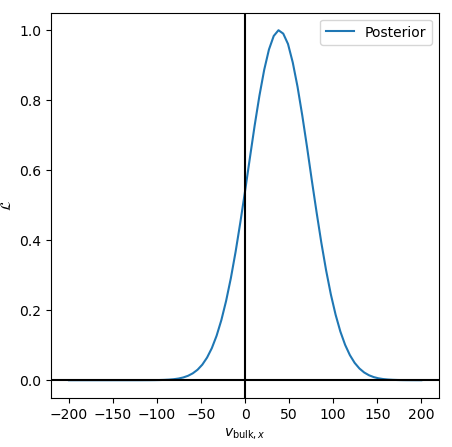
\includegraphics[width=\textwidth]{MainLayout/BORG_chapter/figures/bulk_x_L.png}
        \caption{Likelihood profile for $V_z$}
        \label{fig:Vz_lpt_L}
    \end{subfigure}
    \caption{Likelihood profiles $V_z$ and $V_z$ for a synthetic N-body simulation generated with LPT}
    \label{fig:params3_lpt_L}
\end{figure}

\subsection{Supernova prior improvement $-$ Towards a realistic description of supernovae}

Recent results from \cite{Lordet_2026} have shown that supernovae tend to be found in overly dense regions in the Universe with a large number of supernovae being present at a 
redshift of $z \approx 0.02-0.03$ creating what we see as a "bump" in the supernovae distribution accross redshift. This means that the assumption that the supernovae density is 
constant at low redshift (example of what was done in \cite{Perley_2020}) is not the most accurate description of the supernova distribution. We aimed at trying to account for such 
effects in our model description. We propose a slightly modified version of the supernova prior based on the observed supernova count. The number of supernova 
$N_{\text{SN}}$ observed by a survey between a distance $r$ and $r+dr$ can be expressed as:
\begin{equation}
    dN = n(r) \times 4 \pi r^2 dr
\end{equation}
where $n(r)$ is the number density of supernovae. This can be related to the observed rate as:
\begin{equation}
    R(r) = \mathrm{S}(\phi, \theta, r) \frac{n(r)}{T_{\text{obs}}}
\end{equation}
where $T_{\text{obs}}$ is the time of observation and $\mathrm{S}$ is a selection function that would account for the survey's footprint, galactic extinction and any 
instrumental effects that would decrease the number of observed supernova. Since we are working with the volume limited sample and are 
generating supernova on the full-sky $\mathrm{S}$ becomes unity. 
If we assume a constant rate, then $dN \propto r^2 dr$ giving the $r^2$ geometric dependence in the prior described earlier in Chapter 5 with the self consistent simulations. If we 
assume that this is not the case, then we get:
\begin{equation}
    dN(r) \propto n(r)r^2 dr
\end{equation}
In practice, we do not have direct access to $n(r)$ but we can infer $n(z)$. In Figure (ref) we show the $n(z)$ distribution obtained on the ZTF simulations obtained in 
100? bins up to a redshift of $z=0.06$. We proceed to then fit the number density with a cubic spline. The purpose of fitting with a cubic spline is to keep the $n(z)$ 
differentiable as it will be needed to then infer $n(r)$. In fact, we can relate the two number densities with:
\begin{equation}
    n(r) \propto \frac{n(z)}{4\pi r^2 \times \frac{dr}{dz}}
\end{equation}
The $\frac{dr}{dz}$ term can be deduced from Equation \ref{eqn:physical_distance} and is entirely determined by the cosmology. We get $\frac{dr}{dz} = \frac{c}{H(z)}$
Finally, we can present a more realistic prior on supernovae expressed as:
\begin{equation}
    p(r) \propto r^2\, n(r)\,(1+\delta^F)^{\alpha},
    \quad \text{with } n(r) \propto \frac{n(z)}{4\pi r^2 \times \frac{dr}{dz}}.
\end{equation}

*** We need to test this on both a constant rate simulation and a none constant rate ***